\documentclass[../../main.tex]{subfiles}

\begin{document}
\section{Mutual Information in Markov Chains}
\subsection{Exponential Decay in Irreducible Aperiodic Markov Chains}
    \noindent
    If we have a Markov chain defined by the matrix $\boldsymbol{M}$ (we adopt the notation in the paper and write $\bm{M}$ instead of $\bm{P}$), which is \emph{irreducible} and \emph{aperiodic}, and has a finite state space $S = \{1, \dots, n\}$, then we have that
    \[
        \lim_{i \to \infty} \boldsymbol{M}^i = \boldsymbol{M}_{\boldsymbol{\mu}} \quad ,
    \]
    where $\boldsymbol{M_\mu}$ is the matrix whose columns all consist of the unique stationary probability distribution $\boldsymbol{\mu}$.

    ~\\
    Now, let us consider two random variables $X$ and $Y$, which will denote the state of the Markov chain at times $t_0$ and $t_0 + \tau$ respectively. We assume that we measure these variables very late in the process, where we already have that $\boldsymbol{M}^{t_0} \approx \boldsymbol{M}_{\boldsymbol{\mu}}$. We will use this "equality" later.

    ~\\
    Our goal now is to quantify the mutual information of $X$ and $Y$, that is, the discrepancy between the joint probability distribution $P(X, Y)$ and the one defined by the product of the two marginalized distributions, that is $P'(X, Y) \coloneqq P(X) \cdot P(Y)$. We use the Kullback-Leibler divergence, so our target expression becomes
    \[
        D(P(X, Y) \,\|\, P'(X, Y)) \quad .
    \]

    \smallskip \noindent
    Note that of course this divergence $I(X, Y) \coloneqq D(P(X, Y) \,\|\, P'(X, Y))$ depends on the properties of $M$, as well as on $\tau$. Because $\boldsymbol{M}$ is irreducible and aperiodic, it follows that $|\lambda_2| < 1$. The claim is that
    \[
        I(X, Y) \in \mathcal{O}(|\lambda_2|^\tau) \quad .
    \]
    
    \bigskip \noindent
    There is a lot of math involved, so let us first get an intuition for what is going on. When considering Markov chains, we consider a set of states, say $S = \{A, B, C\}$, and for each time $t \in \mathbb{N}$ we assign a probability to the random variable $X_t \in S$. So let us consider the following Markov chain in figure~\ref{fig:2_markov_chain}.

    \begin{figure}[h]
    \center
    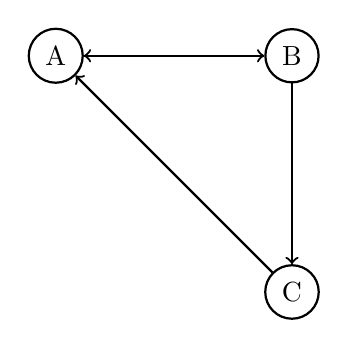
\begin{tikzpicture}[->, auto, node distance=3cm, thick]
    % Define states
    \node[circle, draw] (A) {A};
    \node[circle, draw, right of=A] (B) {B};
    \node[circle, draw, below of=B] (C) {C};

    % Transitions between states
    \draw (A) edge (B);
    \draw (B) edge (A);
    \draw (B) edge (C);
    \draw (C) edge (A);

    % Self-loops
    % \draw (A) edge[loop above] (A);
    % \draw (B) edge[loop above] (B);
    % \draw (C) edge[loop below] (C);

    \end{tikzpicture}
    \caption{A simple irreducible aperiodic Markov chain. Note that if $X_{t_0} = C$, then we know that $X_{t_0+1} = A$.}
    \label{fig:2_markov_chain}
    \end{figure}

    \noindent
    If $\tau = 1$, i.e. we consider the mutual information of to consecutive states, we get a large value of $I(X, Y)$, as if $X_{t_0}$ is either $A$ or $C$, then $X_{t_0+1}$ is uniquely determined, so we have a strong dependency between the two random variables. If, however, we have $\tau = 5$, then we can reach every state independent of the starting position. To see this, note that we can reach every state from $A$ in four steps:
    \begin{itemize}
        \item $A \rightarrow B \rightarrow C \rightarrow A \rightarrow B$
        \item $A \rightarrow B \rightarrow A \rightarrow B \rightarrow C$
        \item $A \rightarrow B \rightarrow A \rightarrow B \rightarrow A$
    \end{itemize}
    The last step can then be used to go around in a cycle. If we on the other hand started at $B$ or $C$, then we could go to $A$ in one step, and consequently to every other state in the following four. Hence, the probability distribution will "wash out" over time and converge to the stationary one, which results in a decline of $I(X, Y)$ for increasing $\tau$.
    
    ~\\
    Because we measure our $X$ very late in time, meaning $t_0$ is very large, we will have that $P(X = a) \approx \boldsymbol{\mu}_a$ because of this "washing out". Similarly, we have $P(Y = b) \approx \boldsymbol{\mu}_b$, since the probability distribution will only get attracted more towards $\boldsymbol{\mu}$. As we now increase $\tau$, $P(Y = b \,|\, X = a)$ itself will converge to $\boldsymbol{\mu}_b$ exactly due to the same "washing out" reason. Note that $P(Y = b \,|\, X = a) = (\boldsymbol{M}^{\tau})_{ba} \xrightarrow{\tau \to \infty}  \boldsymbol{\mu}_b$. And, of course, if $P(X = a, Y = b) = P(X = a) \cdot P(Y = b \,|\, X = a) = \boldsymbol{\mu}_a \cdot \boldsymbol{\mu}_b$, we have $I(X, Y) = 0$. Hence, in a sense the theorem describes how fast $\boldsymbol{M}^{\tau}\bm{p}_0$ converges to $\boldsymbol{\mu}$, or, equivalently, $\boldsymbol{M}^{\tau}$ towards $\boldsymbol{M}_{\boldsymbol{\mu}}$.

    \bigskip \bigskip \noindent
    Now it's time to dive into the math. In the following, we try to reconstruct the arguments given in the paper. We also adopt the notation $P (a, b) \equiv P (X = a, Y = b)$. By definition of the Kullback-Leibler divergence, we have
    \begin{align*}
        D(P(X, Y) \,\|\, P'(X, Y)) &= \sum_{(a,b) \in S^2} P(a, b) \log_B \frac{P(a, b)}{P(a) P(b)} \quad .
    \end{align*}
    The idea is now that $log_B(\bullet)$ is \emph{concave}. Hence, we can upper bound it by its Taylor expansion of the first degree at the point $x_0 = 1$:
    \begin{align*}
        \log_B(x) &\leq \log_B(x_0) + \log_B'(x_0) (x - x_0) \\
        &= 0 + \frac{\ln'(x_0)}{\ln(B)} (x - 1) \\
        &= \frac{\frac{1}{x_0}}{\ln(B)} (x - 1) \\
        &= \frac{x - 1}{\ln(B)} \quad .
    \end{align*}
    For simplicity, we set $B \coloneqq e$. So our expression becomes
    \begin{align*}
        D(P(X, Y) \,\|\, P'(X, Y)) &\leq \frac{1}{\ln(B)}\sum_{(a,b) \in S^2} P(a, b) \left( \frac{P(a, b)}{P(a) P(b)} - 1 \right) \\
        &= \sum_{(a,b) \in S^2} P(a, b) \left( \frac{P(a, b)}{P(a) P(b)} - 1 \right) \\
        &= \left( \sum_{(a,b) \in S^2} P(a, b) \frac{P(a, b)}{P(a) P(b)} \right) - 1 \\
        &= \left( \sum_{(a,b) \in S^2} \frac{P(a, b)^2}{P(a) P(b)} \right) - 1 \\
        &\eqqcolon I_R(X, Y) \quad .
    \end{align*}
    The authors of the paper coin this definition for $I_R(X, Y)$ the \emph{rational mutual information}, as it has some useful properties. As discussed, we can approximate $P(a) \approx \boldsymbol{\mu}_a$ and $P(b) \approx \boldsymbol{\mu}_b$, and also $P(b \,|\, a) = (\boldsymbol{M}^{\tau})_{ba}$. Thus:
    \begin{align*}
        I_R(X, Y) + 1 &= \sum_{(a,b) \in S^2} \frac{P(a, b)^2}{P(a) P(b)} \\
        &= \sum_{(a,b) \in S^2} \frac{P(b \,|\, a)^2 P(a)^2}{P(a) P(b)} \\
        &= \sum_{(a,b) \in S^2} \frac{\boldsymbol{\mu}_a}{\boldsymbol{\mu}_b} \left[ (\boldsymbol{M}^{\tau})_{ba} \right] ^2 \quad .
    \end{align*}
    Let us now focus on $(\boldsymbol{M}^{\tau})_{ba}$. For simplicity, we consider the case that $\boldsymbol{M}$ is diagonalizable (for the general case see section~\ref{section:the_defectvie_case}). Note that since M is irreducible and aperiodic, we have that $1 = \lambda_1 > |\lambda_2| \geq \dots \geq |\lambda_n|$. Hence, let
    \[
        \boldsymbol{M} = \boldsymbol{BDB}^{-1}
    \]
    be the diagonalization of $\boldsymbol{M}$. Of course, we immediately see that $\boldsymbol{M}^\tau = \boldsymbol{BD}^\tau \boldsymbol{B}^{-1}$. Hence, it is easy to verify that
    \[
        (\boldsymbol{M}^\tau)_{ba} = \sum_{c = 1}^{n} \lambda_c^\tau \boldsymbol{B}_{bc}(\boldsymbol{B}^{-1})_{ca} \quad .
    \]

    \bigskip \noindent
    Okay, that was a lot of math. Now it is a good time to reassure ourselves what we actually have achieved. What do we expect $(\boldsymbol{M}^\tau)_{ba}$ to look like for $\tau \rightarrow \infty$? $\boldsymbol{\mu}_b$ of course. What does $\boldsymbol{B}$ look like? Well, this is very hard to tell, it at least should have a scaled version of $\boldsymbol{\mu}$ in its first column. But we cannot really infer any information about $\boldsymbol{B}^{-1}$. But we know
    \begin{align*}
        \boldsymbol{\mu}_b &= \lim_{\tau \to \infty} (\boldsymbol{M}^\tau)_{ba} \\
        &= \lim_{\tau \to \infty} \sum_{c = 1}^{n} \lambda_c^\tau \boldsymbol{B}_{bc}(\boldsymbol{B}^{-1})_{ca} \\
        &= \lambda_1 \boldsymbol{B}_{b1}(\boldsymbol{B}^{-1})_{1a} \quad .
    \end{align*}
    So we know that
    \[
        (\boldsymbol{M}^\tau)_{ba} = \boldsymbol{\mu}_b \pm \mathcal{O}(|\lambda_2|^\tau) \quad .
    \]
    Note that this is informal writing. It would be more precise to state that $|(\boldsymbol{M}^\tau)_{ba} - \boldsymbol{\mu}_b| \in \mathcal{O}(|\lambda_2|^\tau)$.

    ~\\
    This is looking promising, as this means that the discrepancy between $(\boldsymbol{M}^\tau)_{ba}$ and $\boldsymbol{\mu}_b$ decays exponentially. The only thing left to do is translating this exponential decay to the mutual independence measure $I_R(X, Y)$. To this end, we plug our results back into our previous equation. Thus:
    \begin{align*}
        I_R(X, Y) &= \left( \sum_{(a,b) \in S^2} \frac{\boldsymbol{\mu}_a}{\boldsymbol{\mu}_b} \left[ (\boldsymbol{M}^{\tau})_{ba} \right] ^2 \right) - 1 \\
        &= \sum_{(a,b) \in S^2} \left( \frac{\boldsymbol{\mu}_a}{\boldsymbol{\mu}_b} \left[ (\boldsymbol{M}^{\tau})_{ba} \right] ^2 - \boldsymbol{\mu}_a \boldsymbol{\mu}_b \right) \\
        &= \sum_{(a,b) \in S^2} \left( \frac{\boldsymbol{\mu}_a}{\boldsymbol{\mu}_b} \left[ \boldsymbol{\mu}_b \pm \mathcal{O}(|\lambda_2|^\tau) \right] ^2 - \boldsymbol{\mu}_a \boldsymbol{\mu}_b \right) \\
        &= \sum_{(a,b) \in S^2} \left( \frac{\boldsymbol{\mu}_a}{\boldsymbol{\mu}_b} \left[ \boldsymbol{\mu}_b^2 \pm \mathcal{O}(|\lambda_2|^\tau) \right] - \boldsymbol{\mu}_a \boldsymbol{\mu}_b \right) \\
        &= \pm \sum_{(a,b) \in S^2} \frac{\boldsymbol{\mu}_a}{\boldsymbol{\mu}_b} \mathcal{O}(|\lambda_2|^\tau) \quad , \\
    \end{align*}
    where we have used multiple facts about $\boldsymbol{\mu}$. For instance, $\sum_{a \in S} \boldsymbol{\mu}_a = 1$ and thus $\sum_{(a,b) \in S^2} \boldsymbol{\mu}_a \boldsymbol{\mu}_b = 1$, as well as $0 < \boldsymbol{\mu}_a < 1$ for all $a \in S$ (at least for $|S| > 1$). We now use the latter inequality again: We see that we can always bound $\frac{\boldsymbol{\mu}_a}{\boldsymbol{\mu}_b}$ from above, i.e. there exists $\alpha \in \mathbb{R}$ s.t. for all $(a,b) \in S^2$ we have $\frac{\boldsymbol{\mu}_a}{\boldsymbol{\mu}_b} < \alpha$. Hence:

    \begin{align*}
        &|I_R(X, Y)| \in \sum_{(a,b) \in S^2} \frac{\boldsymbol{\mu}_a}{\boldsymbol{\mu}_b} \mathcal{O}(|\lambda_2|^\tau) \\
        &\implies |I_R(X, Y)| \in \sum_{(a,b) \in S^2} \alpha \mathcal{O}(|\lambda_2|^\tau) \\
        &\implies |I_R(X, Y)| \in n^2 \alpha \mathcal{O}(|\lambda_2|^\tau) \\
        &\implies |I_R(X, Y)| \in \mathcal{O}(|\lambda_2|^\tau) \quad .
    \end{align*}
    Of course, $I_R(X, Y) \geq 0$, so really $I_R(X, Y) \in \mathcal{O}(|\lambda_2|^\tau)$. Since $0 \leq I(X, Y) \leq I_R(X, Y)$, we also have $I(X, Y) \in \mathcal{O}(|\lambda_2|^\tau)$.

    \bigskip
    \begin{remark}
        The above proof should also work without the approximation $P(a) \approx \bm{\mu}_a$, so $t_0$ musn't be big.
    \end{remark}

    \begin{remark}
        Based on the proof, we see that if the distance between $\bm{M}^\tau$ and $\bm{M_\mu}$ experiences exponential decay, we can translate this exponential decay to the mutual information measure $I_R(X, Y)$. Note that we have already established that \emph{all} irreducible aperiodic Markov chains have this property in remark~\ref{remark:exponential_decay}.
    \end{remark}

\subsubsection{The Defective Case}
    \label{section:the_defectvie_case}
    Nonetheless, we will prove the case that $\bm{M}$ is not diagonalizable separately and establish the connection to $\lambda_2$. The idea is that while not every matrix is diagonalizable, every square matrix over the complex numbers can be put into \emph{Jordan normal form}, which resembles diagonalization. In this form, the matrix is nearly diagonal, except that for each repeated eigenvalue, there may be 1s on the superdiagonal (just above the main diagonal), indicating the presence of generalized eigenvectors.

    For example, if there are only three distinct eigenvalues and $\lambda_2$ is threefold degenerate, the the Jordan form of $\bm{M}$ would be
    \[
        \bm{B}^{-1}\bm{MB} =
        \begin{bmatrix}
        \lambda_1 & 0 & 0 & 0 & 0 \\
        0 & \lambda_2 & 1 & 0 & 0 \\
        0 & 0 & \lambda_2 & 1 & 0 \\
        0 & 0 & 0 & \lambda_2 & 0 \\
        0 & 0 & 0 & 0 & \lambda_3 \\
        \end{bmatrix}
        \eqqcolon \bm{D}
        \quad .
    \]
    Thus, again $\bm{M}^\tau = \bm{BD}^\tau \bm{B}^{-1}$, and the claim is that for our example $\bm{D}^\tau$ reads as
    \[
        \bm{D} =
        \begin{bmatrix}
        1 & 0 & 0 & 0 & 0 \\
        0 & \lambda_2^\tau & \binom{\tau}{1} \lambda_2^{\tau - 1} & \binom{\tau}{2} \lambda_2^{\tau - 2} & 0 \\
        0 & 0 & \lambda_2^\tau & \binom{\tau}{1} \lambda_2^{\tau - 1} & 0 \\
        0 & 0 & 0 & \lambda_2^\tau & 0 \\
        0 & 0 & 0 & 0 & \lambda_3^\tau \\
        \end{bmatrix}
        \quad .
    \]
    All the entries except the ones in the blocks with the binomial coefficient terms are trivial. So let us quickly verify those. For $\tau \coloneqq 1$ it obviously holds when setting $\binom{\tau}{n} \coloneqq 0$ for $n > \tau$. So assume the claim holds for $\tau \coloneqq k$. Then we have
    \begin{align*}
        \bm{D}^{k + 1} &= \bm{D}^k \bm{D} \\
        &=
        \begin{bmatrix}
        1 & 0 & 0 & 0 & 0 \\
        0 & \lambda_2^k & \binom{k}{1} \lambda_2^{k - 1} & \binom{k}{2} \lambda_2^{k - 2} & 0 \\
        0 & 0 & \lambda_2^k & \binom{k}{1} \lambda_2^{k - 1} & 0 \\
        0 & 0 & 0 & \lambda_2^k & 0 \\
        0 & 0 & 0 & 0 & \lambda_3^k \\
        \end{bmatrix}
        \begin{bmatrix}
        \lambda_1 & 0 & 0 & 0 & 0 \\
        0 & \lambda_2 & 1 & 0 & 0 \\
        0 & 0 & \lambda_2 & 1 & 0 \\
        0 & 0 & 0 & \lambda_2 & 0 \\
        0 & 0 & 0 & 0 & \lambda_3 \\
        \end{bmatrix}
        \quad . \\
    \end{align*}
    Thus, at $j \geq i, \ d \coloneqq j - i$, $(\bm{D}^k)_{i,j} = \binom{k}{d} \lambda_2^{k - d}$, and hence we have
    \begin{align*}
        (\bm{D}^{k + 1})_{i,j} &= (\bm{D}^k)_{i, j - 1} (\bm{D})_{j - 1, j} + (\bm{D}^k)_{i, j} (\bm{D})_{j, j} \\
        &= (\bm{D}^k)_{i, i + (d - 1)} + (\bm{D}^k)_{i, i + d} \lambda_2 \\
        &= \binom{k}{d - 1} \lambda_2^{k - d + 1} + \binom{k}{d} \lambda_2^{k - d} \lambda_2 \\
        &= \binom{k}{d - 1} \lambda_2^{k - d + 1} + \binom{k}{d} \lambda_2^{k - d + 1} \\
        &= \left( \binom{k}{d - 1} + \binom{k}{d} \right) \lambda_2^{k - d + 1} \\
        &\overset{\checkmark}{=} \binom{k + 1}{d} \lambda_2^{k + 1 - d} \quad ,
    \end{align*}
    just as expected.

    This was just an example, but it is easy to see that we can generalize this, and we get that the absolute value of every entry in $\bm{D}^\tau$, except the top left 1, is $\mathcal{O}(|\lambda_2^+|^\tau)$, where $\lambda_2^+$ is defined s.t. $|\lambda_2^+| = |\lambda_2| + \epsilon$ for some $\epsilon \in \mathbb{R}_{>0}$. Note that $|\binom{\tau}{d} \lambda_2^{\tau - d}| \in \mathcal{O}(|\lambda_2^+|^\tau)$ for each $d \in \mathbb{N}$.

    The rest is trivial, as all the the entries in $\bm{B}$ and $\bm{B}^{-1}$ are really just constants, and hence when calculating $(\bm{M}^\tau)_{ba} = (\bm{BD}^\tau\bm{B}^{-1})_{ba}$, we have
    \begin{align*}
        (\bm{BD}^\tau\bm{B}^{-1})_{ba} &= \left( \bm{B} \left(
            \begin{bmatrix}
            1      & 0      & \cdots & 0 \\
            0      & 0      & \cdots & 0 \\
            \vdots & \vdots & \ddots & \vdots \\
            0      & 0      & \cdots & 0
            \end{bmatrix}
            +
            \begin{bmatrix}
            c_{11} & c_{12} & \cdots & c_{1n} \\
            c_{21} & c_{22} & \cdots & c_{2n} \\
            \vdots & \vdots & \ddots & \vdots \\
            c_{n1} & c_{n2} & \cdots & c_{nn}
            \end{bmatrix}
            \mathcal{O}(|\lambda_2^+|^\tau)
        \right)
        \bm{B}^{-1} \right)_{ba} \\
        &= \bm{\mu}_b \pm \mathcal{O}(|\lambda_2^+|^\tau)
        \quad ,
    \end{align*}
    for some $c_{ij} \in \mathbb{C}, \ |c_{ij}| = 1$. The rest of the proof is identical to the one given.

\subsection{No Markov Chain with Power-Law Decay}
    We are interested in cases where $I(X, Y)$ decays to $0$, as this is implied by a power-law decay. This means that for increasing $\tau$, we get in the limit $\tau \to \infty$ that $P(a, b) = P(a) P(b \mid a) = P(a) (\bm{M}^\tau)_{ba} \overset{!}{=} P(a) P(b)$, and hence $(\bm{M}^\tau)_{ba} = P(b)$ for every $a \in S$. Clearly, this means that $\bm{M}^\tau$ must converge to a stationary matrix $\bm{M_\mu}$, where all columns are equal, at least given the case that $P(b)$ converges for all $b \in S$. But thanks to the following lemma, we can assume that this is the case:

    \begin{lemma}[Convergence of P(b) is Necessary for Power-Law Decay]
        In order for $I(X, Y)$ to converge to $0$ for increasing $\tau$, we must have that $\lim_{t \to \infty}\bm{M}^t \bm{p}_0 = \bm{\mu}$ for every $\bm{p}_0 \in \Delta$ (and hence $P(b)$ converges).
    \end{lemma}
    \vspace{-2.5em}
    \begin{proof}
        In order for $I(X, Y)$ to converge to $0$, we still must have that $|(\bm{M}^\tau)_{ba} - P(X_{t_0 + \tau} = b)| \xrightarrow{\tau \to \infty} 0$ for every $a \in S$. But note that for this to happen we must have close to equal columns for increasing $\tau$, because $(\bm{M}^\tau)_{ba}$ must be independent of $a$. But such a matrix must be stationary (and hence $P(b)$ converges), so we cannot have $I(X, Y) = 0$ if $P(b)$ does not converge.
    \end{proof}

    \begin{theorem}[No Markov Chain with Power-Law Decay]
        There is no Markov chain $\bm{M}$ with $I(X_{t_0}, X_{t_0 + \tau}) \in \mathcal{O}(\tau^{-\alpha})$ and $I(X_{t_0}, X_{t_0 + \tau}) \in \Omega (\tau^{-\beta})$ for some $\alpha, \beta \in \mathbb{R}_{>0}$.
    \end{theorem}
    \vspace{-2.5em}
    \begin{proof}
        For the sake of contradiction, assume that $\bm{M}$ produces power-law decay. Due to the previous results, we know that $\bm{M}^\tau$ converges to a stationary matrix $\bm{M_\mu}$. (The following discussion is facultative; it aims to enhance the reader's understanding). $\bm{M_\mu}$ must contain 0-entries, as if it didn't, it would mean that $\bm{M}$ is irreducible and aperiodic based on corollary~\ref{corollary:converse_positive_transition_matrix}, and hence $\bm{M}$ would have exponential decay.

        Thus, let's focus on all the rows of $\bm{M_\mu}$ with non-0-entries with associated states $S_C$. We see that for all $i \in S_C, j \in S$ we have that $(\bm{M_\mu})_{ij} > 0$ (especially for $j \in S_C$). Hence, the set $S_C$ describes a closed communication class. Furthermore, there cannot be another closed communication class, since in a closed communication class the transition probabilities between any two states cannot approach 0. Thus, all other states $S \setminus S_C \eqqcolon S_O$ are in an open communication class.
        
        For indexing reasons, we assume without loss of generality that $S_C = \{ 1, \dots, n' \} \subseteq S$.
        Since $S_C$ is a closed communication class, we have that for all $j \in S_C, i \in S_O, t \in \mathbb{N}_{>0}: (\bm{M}^t)_{ij} = 0$ (especially for $t \coloneqq 1$). Thus for all $i,j \in S_C, t \in \mathbb{N}_{>0}$:
        \begin{align*}   
            (\bm{M}^{t+1})_{ij} &= (\bm{M}^t \bm{M})_{ij} \\
            &= \sum_{k \in S} (\bm{M}^t)_{ik} (\bm{M})_{kj} \\
            &= \sum_{k \in S_C} (\bm{M}^t)_{ik} (\bm{M})_{kj} \quad .
        \end{align*}
        Now, let $\bm{M}_{S_C}$ be the sub-matrix of $\bm{M}$ containing and only containing the transition probability entries for the states in $S_C$ (with our assumption $\bm{M}_{S_C}$ is the top left sub-matrix of $\bm{M}$). From our result, we see that $(\bm{M}^t)_{S_C} = (\bm{M}_{S_C})^t$.

        But $(\bm{M}^t)_{S_C}$ converges to a positive matrix, and hence so must $(\bm{M}_{S_C})^t$. Hence, $\bm{M}_{S_C}$ must be irreducible aperiodic based on corollary~\ref{corollary:converse_positive_transition_matrix} again. Thus, $(\bm{M}_{S_C})^t$ converges with exponential decay (with a basis of $|\lambda_2| < 1$ of $\bm{M}_{S_C}$), and hence so does $(\bm{M}^t)_{S_C}$.

        Quickly note that $\lambda_2$ of $\bm{M}_{S_C}$ is an eigenvalue of $\bm{M}$ as well: There must be (at least) one associated eigenvector $v \in \mathbb{C}^{|S_C|}$ s.t. $\bm{M}_{S_C} v = \lambda_2 v$. Now, extend $v$ to an eigenvector $v'$ of $\bm{M}$ by adding zeros in all the places associated with states in $S_O$ (here: at the end). For $i \in S_C$ we have:
        \begin{align*}
            (\bm{M} v')_i &= \sum_{j \in S} \bm{M}_{ij} v'_j \\
            &\underset{\text{0-entries of v'}}{=} \sum_{j \in S_C} \bm{M}_{ij} v'_j \\
            &= \sum_{j \in S_C} \bm{M}_{ij} v_j \\
            &\underset{i \in S_C}{=} \sum_{j \in S_C} (\bm{M}_{S_C})_{ij} v_j \\
            &= (\bm{M}_{S_C} v)_i \\
            &= \lambda_2 v_i \overset{\checkmark}{=} \lambda_2 v'_i \quad ,
        \end{align*}
        and for $i \in S_O$ it follows that
        \begin{align*}
            (\bm{M} v')_i &= \sum_{j \in S} \bm{M}_{ij} v'_j \\
            &\underset{\text{0-entries of v'}}{=} \sum_{j \in S_C} \bm{M}_{ij} v'_j \\
            &\underset{i \in S_O}{=} \sum_{j \in S_C} 0 \cdot v'_j \\
            &= 0 \overset{\checkmark}{=} \lambda_2 v'_i \quad .
        \end{align*}

        The only things left to do are, first, to verify that $|\lambda_2|$ of $\bm{M}_{S_C}$ is less than or equal to the absolute value of the second largest eigenvalue of $\bm{M}$; and second, to show the convergence of $\bm{M}_{S_O}$ and that it also exhibits exponential decay (with a base less than or equal to $|\lambda_2|$ of $\bm{M}$). Luckily, we achieve all our goals thanks to the following observation:

        (Start of the actual proof.) Since $\bm{M}^t$ converges to $\bm{M_\mu}$, there must exist an $m \in \mathbb{N}_{>0}$ s.t. $\bm{M}^m$ and $\bm{M}^{m + 1}$ both have a positive row. Thus, thanks to corollary~\ref{corollary:perron_frobenius_extension} we can apply the Perron-Frobenius Theorem (with the exception that the eigenvector must not be positive) to $\bm{M}^m$ and $\bm{M}^{m + 1}$, and thanks to lemma~\ref{lemma:perron_frobenius_extension_A_to_the_m} also to $\bm{M}$ itself. Of course, $\lambda_{max} = 1$ with the associated eigenvector $\bm{\mu}$. So we know that $|\lambda_2| < 1$ of $\bm{M}_{S_C}$ is less than or equal to the absolute value of the second largest eigenvalue of $\bm{M}$.

        Furthermore, we of course have that $\lim_{\tau \to \infty} (\bm{M}^\tau)_{ba} = \bm{\mu}_b \ (\coloneqq \lim_{\tau \to \infty} P(b))$. But those were the only two assumptions made in section~\ref{section:the_defectvie_case}. Thus, by the same logic, we get $I(X_{t_0}, X_{t_0 + \tau}) \in \mathcal{O}(|\lambda_2^+|^\tau)$.
    \end{proof}
\end{document}